\documentclass{article}\usepackage[]{graphicx}\usepackage[]{xcolor}
% maxwidth is the original width if it is less than linewidth
% otherwise use linewidth (to make sure the graphics do not exceed the margin)
\makeatletter
\def\maxwidth{ %
  \ifdim\Gin@nat@width>\linewidth
    \linewidth
  \else
    \Gin@nat@width
  \fi
}
\makeatother

\definecolor{fgcolor}{rgb}{0.345, 0.345, 0.345}
\newcommand{\hlnum}[1]{\textcolor[rgb]{0.686,0.059,0.569}{#1}}%
\newcommand{\hlsng}[1]{\textcolor[rgb]{0.192,0.494,0.8}{#1}}%
\newcommand{\hlcom}[1]{\textcolor[rgb]{0.678,0.584,0.686}{\textit{#1}}}%
\newcommand{\hlopt}[1]{\textcolor[rgb]{0,0,0}{#1}}%
\newcommand{\hldef}[1]{\textcolor[rgb]{0.345,0.345,0.345}{#1}}%
\newcommand{\hlkwa}[1]{\textcolor[rgb]{0.161,0.373,0.58}{\textbf{#1}}}%
\newcommand{\hlkwb}[1]{\textcolor[rgb]{0.69,0.353,0.396}{#1}}%
\newcommand{\hlkwc}[1]{\textcolor[rgb]{0.333,0.667,0.333}{#1}}%
\newcommand{\hlkwd}[1]{\textcolor[rgb]{0.737,0.353,0.396}{\textbf{#1}}}%
\let\hlipl\hlkwb

\usepackage{framed}
\makeatletter
\newenvironment{kframe}{%
 \def\at@end@of@kframe{}%
 \ifinner\ifhmode%
  \def\at@end@of@kframe{\end{minipage}}%
  \begin{minipage}{\columnwidth}%
 \fi\fi%
 \def\FrameCommand##1{\hskip\@totalleftmargin \hskip-\fboxsep
 \colorbox{shadecolor}{##1}\hskip-\fboxsep
     % There is no \\@totalrightmargin, so:
     \hskip-\linewidth \hskip-\@totalleftmargin \hskip\columnwidth}%
 \MakeFramed {\advance\hsize-\width
   \@totalleftmargin\z@ \linewidth\hsize
   \@setminipage}}%
 {\par\unskip\endMakeFramed%
 \at@end@of@kframe}
\makeatother

\definecolor{shadecolor}{rgb}{.97, .97, .97}
\definecolor{messagecolor}{rgb}{0, 0, 0}
\definecolor{warningcolor}{rgb}{1, 0, 1}
\definecolor{errorcolor}{rgb}{1, 0, 0}
\newenvironment{knitrout}{}{} % an empty environment to be redefined in TeX

\usepackage{alltt}
\usepackage[margin=1.0in]{geometry} % To set margins
\usepackage{amsmath}  % This allows me to use the align functionality.
                      % If you find yourself trying to replicate
                      % something you found online, ensure you're
                      % loading the necessary packages!
\usepackage{amsfonts} % Math font
\usepackage{fancyvrb}
\usepackage{hyperref} % For including hyperlinks
\usepackage[shortlabels]{enumitem}% For enumerated lists with labels specified
                                  % We had to run tlmgr_install("enumitem") in R
\usepackage{float}    % For telling R where to put a table/figure
\usepackage{natbib}        %For the bibliography
\bibliographystyle{apalike}%For the bibliography
\IfFileExists{upquote.sty}{\usepackage{upquote}}{}
\begin{document}


\cite{Kasdin25} show that dopamine in the brains of young zebra finches acts as 
a learning signal, increasing when they sing closer to their adult song and 
decreasing when they sing further away, effectively guiding their vocal 
development through trial-and-error. This suggests that complex natural 
behaviors, like learning to sing, are shaped by dopamine-driven reinforcement 
learning, similar to how artificial intelligence learns. You can find the 
paper at this link:
\href{https://www.nature.com/articles/s41586-025-08729-1}{{https://www.nature.com/articles/s41586-025-08729-1}.}.

Note they measure dopamine using fibre photometry, changes in the fluorescence
indicate dopamine changes in realtime. Their specific measurement considers 
changes in flourescence in 100-ms windows between 200 and 300 ms from the start 
of singing, averaged across development.

\begin{enumerate}
%%%%%%%%%%%%%%%%%%%%%%%%%%%%%%%%%%%%%%%%%%%%%%%%%%%%%%%%%%%%%%%%%
% CONDUCT A POWER ANALYSIS
%%%%%%%%%%%%%%%%%%%%%%%%%%%%%%%%%%%%%%%%%%%%%%%%%%%%%%%%%%%%%%%%%
\item Using the \texttt{pwr} package for \texttt{R} \citep{pwr},
conduct a power analysis. How many observations would the researchers 
need to detect a moderate-to-large effect ($d=0.65$) when using 
$\alpha=0.05$ and default power (0.80) for a two-sided one sample 
$t$ test.

\begin{knitrout}\scriptsize
\definecolor{shadecolor}{rgb}{0.969, 0.969, 0.969}\color{fgcolor}\begin{kframe}
\begin{alltt}
\hlkwd{library}\hldef{(tidyverse)}
\hlkwd{library}\hldef{(pwr)}

\hldef{power.result} \hlkwb{<-} \hlkwd{power.t.test}\hldef{(}\hlkwc{delta}\hldef{=}\hlnum{0.65}\hldef{,} \hlkwc{sig.level}\hldef{=}\hlnum{0.05}\hldef{,} \hlkwc{power}\hldef{=}\hlnum{0.80}\hldef{,}
                           \hlkwc{type}\hldef{=}\hlsng{"one.sample"}\hldef{,} \hlkwc{alternative}\hldef{=}\hlsng{"two.sided"}\hldef{)}
\hldef{(n.val} \hlkwb{<-} \hldef{power.result}\hlopt{$}\hldef{n)}
\end{alltt}
\begin{verbatim}
## [1] 20.58044
\end{verbatim}
\end{kframe}
\end{knitrout}

To determine the required number of observations to detect a moderate-to-large
effect($d=0.65$) with a significance level of $\alpha=0.05$ and a power
of $0.80$ for a two-sided one-sample t-test, we used the \texttt{pwr} package in 
\texttt{R} \citep{pwr}.The power analysis indicates that approximately 21
observations are needed to reliability detect this effect size. This sample size
would give researchers an $80\%$ chance of correctly rejecting the null hypothesis
when the effect is truly present.

%%%%%%%%%%%%%%%%%%%%%%%%%%%%%%%%%%%%%%%%%%%%%%%%%%%%%%%%%%%%%%%%%
% COLLECT DATA
%%%%%%%%%%%%%%%%%%%%%%%%%%%%%%%%%%%%%%%%%%%%%%%%%%%%%%%%%%%%%%%%%
\item Click the link to go to the paper. Find the source data for 
Figure 2. Download the Excel file. Describe what you needed to
do to collect the data for Figure 2(g). Note that you only need the 
\texttt{closer\_vals} and \texttt{further\_vals}. Ensure to 
\texttt{mutate()} the data to get a difference 
(e.g., \texttt{closer\_vals - further\_vals}).

\begin{knitrout}\scriptsize
\definecolor{shadecolor}{rgb}{0.969, 0.969, 0.969}\color{fgcolor}\begin{kframe}
\begin{alltt}
\hldef{dat} \hlkwb{<-} \hlkwd{read.csv}\hldef{(}\hlsng{"data.csv"}\hldef{)}

\hldef{dat.clean} \hlkwb{<-} \hldef{dat |>}
  \hlkwd{mutate}\hldef{(}\hlkwc{difference} \hldef{= closer_vals} \hlopt{-} \hldef{further_vals)}
\hldef{(dat.clean)}
\end{alltt}
\begin{verbatim}
##    further_vals closer_vals difference
## 1   -0.19168505 0.275714146 0.46739919
## 2   -0.02993474 0.084044448 0.11397919
## 3   -0.18674609 0.131846414 0.31859251
## 4   -0.07381857 0.036630190 0.11044876
## 5   -0.08879365 0.145534134 0.23432778
## 6   -0.16044005 0.195669989 0.35611003
## 7   -0.30926059 0.158454214 0.46771480
## 8   -0.15890017 0.179967148 0.33886732
## 9   -0.12535659 0.131045171 0.25640176
## 10  -0.05447568 0.096865366 0.15134104
## 11  -0.60278594 0.329094427 0.93188037
## 12  -0.23766536 0.169982634 0.40764799
## 13  -0.12270538 0.074888134 0.19759351
## 14  -0.12990904 0.004057814 0.13396685
## 15  -0.04227093 0.001082100 0.04335303
## 16  -0.24306660 0.089018022 0.33208462
## 17  -0.34456488 0.260877405 0.60544228
## 18  -0.31220099 0.276972646 0.58917363
## 19  -0.17620137 0.072787838 0.24898921
## 20  -0.07446303 0.154177639 0.22864067
## 21  -0.34440941 0.266133888 0.61054330
## 22  -0.19040289 0.145314346 0.33571724
## 23  -0.20135921 0.095041639 0.29640085
## 24  -0.31355996 0.190888685 0.50444864
## 25  -0.35313445 0.339488076 0.69262252
\end{verbatim}
\end{kframe}
\end{knitrout}

To collect data for Figure 2(g), we downloaded the Excel file containing the
source data. We extracted only the relevant columns, namely \texttt{closer\_vals}
and \texttt{further\_vals}, corresponding to 2(g), and saved them into a new CSV
file titled \texttt{data.csv} for analysis. After loading the data into \texttt{R},
we used \texttt{mutate()} to create a new column with the calculated difference
between the two conditions (\texttt{closer\_vals - further\_vals}), allowing us to examine
how dopamine signals changed depending on vocal similarity.

%%%%%%%%%%%%%%%%%%%%%%%%%%%%%%%%%%%%%%%%%%%%%%%%%%%%%%%%%%%%%%%%%
% SUMMARIZE DATA
%%%%%%%%%%%%%%%%%%%%%%%%%%%%%%%%%%%%%%%%%%%%%%%%%%%%%%%%%%%%%%%%%
\item Summarize the data.
\begin{enumerate}
  \item Summarize the further data. Do the data suggest that
   dopamine in the brains of young zebra finches decreases when
   they sing further away?
   
\begin{knitrout}\scriptsize
\definecolor{shadecolor}{rgb}{0.969, 0.969, 0.969}\color{fgcolor}\begin{kframe}
\begin{alltt}
 \hldef{summarize.further} \hlkwb{<-} \hldef{dat.clean |>}
   \hlkwd{summarize}\hldef{(}
     \hlkwc{mean} \hldef{=} \hlkwd{mean}\hldef{(further_vals,} \hlkwc{na.rm}\hldef{=T),}
     \hlkwc{sd} \hldef{=} \hlkwd{sd}\hldef{(further_vals,} \hlkwc{na.rm}\hldef{=T)}
   \hldef{)}

 \hldef{(summarize.further)}
\end{alltt}
\begin{verbatim}
##         mean        sd
## 1 -0.2027244 0.1303193
\end{verbatim}
\end{kframe}
\end{knitrout}

  The further data show a mean percent change in fluorescence of $-0.20$ with a
  standard deviation of 0.13, suggesting that dopamine levels tend to decrease 
  when zebra finches sing notes that are further from their adult song. This
  negative mean fluorescence change aligns with the hypothesis that imprecise
  vocalizations lead to lower dopamine levels.
  
   \item Summarize the closer data. Do the data suggest that
   dopamine in the brains of young zebra finches increases when
   they sing closer to their adult song?
   
\begin{knitrout}\scriptsize
\definecolor{shadecolor}{rgb}{0.969, 0.969, 0.969}\color{fgcolor}\begin{kframe}
\begin{alltt}
\hldef{summarize.closer} \hlkwb{<-} \hldef{dat.clean |>}
  \hlkwd{summarize}\hldef{(}
    \hlkwc{mean} \hldef{=} \hlkwd{mean}\hldef{(closer_vals,} \hlkwc{na.rm}\hldef{=T),}
    \hlkwc{sd} \hldef{=} \hlkwd{sd}\hldef{(closer_vals,} \hlkwc{na.rm}\hldef{=T)}
  \hldef{)}

\hldef{(summarize.closer)}
\end{alltt}
\begin{verbatim}
##        mean         sd
## 1 0.1562231 0.09408297
\end{verbatim}
\end{kframe}
\end{knitrout}

The closer data have a mean change in fluorescence of 0.16 with a standard
deviation of 0.09, indicating a consistent increase in dopamine when zebra finches
produce more accurate vocalizations. This relatively low standard deviation also
suggests this effect is robust across individuals.
   
  \item Summarize the paired differences. Do the data suggest
  that there is a difference between dopamine in the brains of
  young zebra finches when they sing further away compared to 
  closer to their adult song?
  
\begin{knitrout}\scriptsize
\definecolor{shadecolor}{rgb}{0.969, 0.969, 0.969}\color{fgcolor}\begin{kframe}
\begin{alltt}
\hldef{summarize.differences} \hlkwb{<-} \hldef{dat.clean |>}
  \hlkwd{summarize}\hldef{(}
    \hlkwc{mean} \hldef{=} \hlkwd{mean}\hldef{(difference,} \hlkwc{na.rm}\hldef{=T),}
    \hlkwc{sd} \hldef{=} \hlkwd{sd}\hldef{(difference,} \hlkwc{na.rm}\hldef{=T)}
  \hldef{)}
\hldef{(summarize.differences)}
\end{alltt}
\begin{verbatim}
##        mean        sd
## 1 0.3589475 0.2108744
\end{verbatim}
\end{kframe}
\end{knitrout}

  The paired differences between closer and further conditions show a mean
  difference of 0.36 and a standard deviation of 0.21. The magnitude of this 
  effect (0.36) relative to the variability (0.21) suggests a strong and meaningful
  difference between the two conditions, potentially supporting the theory that
  learning to sing is shaped by dopamine-driven reinforcement learning.
  
  The boxplot below in Figure \ref{datasummary} visually reinforces this trend, clearly showing that
  fluorescence changes are consistently positive in the closer condition and consistently negative in
  the further condition. The paired differences stand out as they are far above zero, capturing overall
  increase in dopamine signaling. 

\begin{knitrout}\scriptsize
\definecolor{shadecolor}{rgb}{0.969, 0.969, 0.969}\color{fgcolor}
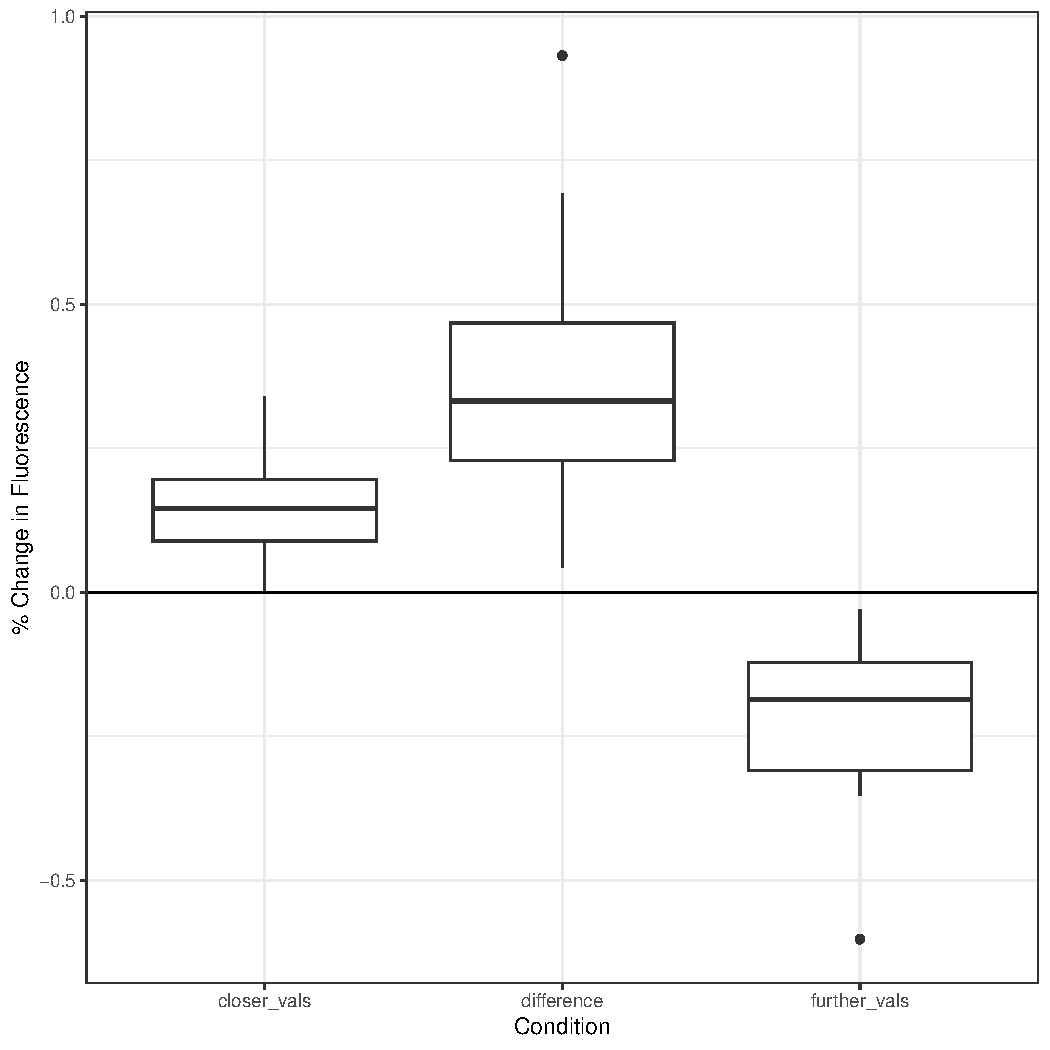
\includegraphics[width=\maxwidth]{figure/plot1-1} 
\end{knitrout}

\begin{figure}[H]
\begin{center}

\caption{$\%$ Change in Flourescence Across Conditions}
\label{datasummary} %we can now reference plot1
\end{center}
\end{figure}


  \item \textbf{Optional Challenge:} Can you reproduce Figure 2(g)?
  Note that the you can use \texttt{geom\_errorbar()} to plot
  the range created by adding the mean $\pm$ one standard deviation.
\end{enumerate}
%%%%%%%%%%%%%%%%%%%%%%%%%%%%%%%%%%%%%%%%%%%%%%%%%%%%%%%%%%%%%%%%%
% CONDUCT THE TESTS
%%%%%%%%%%%%%%%%%%%%%%%%%%%%%%%%%%%%%%%%%%%%%%%%%%%%%%%%%%%%%%%%%
\item Conduct the inferences they do in the paper. Make sure to report the results
a little more comprehensively -- that is your parenthetical should look something
like: ($t=23.99$, $p<0.0001$; $g=1.34$; 95\% CI: 4.43, 4.60).\\
\textbf{Note:} Your numbers may vary slightly as they performed some unclear
correction of their $p$-values. I'm waiting to hear back from them via email!
\begin{enumerate}
  \item ``The close responses differed significantly from 0 ($p=1.63 \times 10^{-8}$).''
  
\begin{kframe}
\begin{alltt}
\hlkwd{library}\hldef{(effectsize)}

\hlcom{# close}
\hldef{hedges_result_closer} \hlkwb{<-} \hlkwd{hedges_g}\hldef{(}\hlkwc{x} \hldef{= dat.clean}\hlopt{$}\hldef{closer_vals,} \hlkwc{mu} \hldef{=} \hlnum{0}\hldef{,} \hlkwc{alternative} \hldef{=} \hlsng{"greater"}\hldef{)}

\hlkwd{help}\hldef{(}\hlsng{"hedges_g"}\hldef{)}

\hldef{t_test_result_closer} \hlkwb{<-} \hlkwd{t.test}\hldef{(}\hlkwc{x}\hldef{=dat.clean}\hlopt{$}\hldef{closer_vals,} \hlkwc{mu} \hldef{=} \hlnum{0}\hldef{,} \hlkwc{alternative} \hldef{=} \hlsng{"greater"}\hldef{)}
\hldef{t_test_result_closer.ci} \hlkwb{<-} \hlkwd{t.test}\hldef{(}\hlkwc{x}\hldef{=dat.clean}\hlopt{$}\hldef{closer_vals,} \hlkwc{mu} \hldef{=} \hlnum{0}\hldef{,} \hlkwc{alternative} \hldef{=} \hlsng{"two.sided"}\hldef{)}

\hldef{t_stat_closer} \hlkwb{<-} \hldef{t_test_result_closer}\hlopt{$}\hldef{statistic}
\hldef{p_val_closer} \hlkwb{<-} \hldef{t_test_result_closer}\hlopt{$}\hldef{p.value}
\hldef{hedges_g_closer} \hlkwb{<-} \hldef{hedges_result_closer}\hlopt{$}\hldef{Hedges_g}
\hldef{ci_low_closer} \hlkwb{<-} \hldef{t_test_result_closer.ci}\hlopt{$}\hldef{conf.int[}\hlnum{1}\hldef{]}
\hldef{ci_high_closer} \hlkwb{<-} \hldef{t_test_result_closer.ci}\hlopt{$}\hldef{conf.int[}\hlnum{2}\hldef{]}

\hldef{results.closer} \hlkwb{<-} \hlkwd{data.frame}\hldef{(}
  \hlkwc{t} \hldef{=} \hlkwd{c}\hldef{(t_stat_closer),}
  \hlkwc{p_value} \hldef{=} \hlkwd{c}\hldef{(p_val_closer),}
  \hlkwc{g} \hldef{=} \hlkwd{c}\hldef{(hedges_g_closer),}
  \hlkwc{CI_Lower} \hldef{=} \hlkwd{c}\hldef{(ci_low_closer),}
  \hlkwc{CI_Upper} \hldef{=} \hlkwd{c}\hldef{(ci_high_closer)}
\hldef{)}

\hlkwd{library}\hldef{(xtable)}
\hldef{results.closer.xtable} \hlkwb{<-} \hlkwd{xtable}\hldef{(results.closer,}
                                \hlkwc{caption}\hldef{=}\hlsng{"Closer Inferences"}\hldef{)}
\end{alltt}
\end{kframe}
% latex table generated in R 4.4.2 by xtable 1.8-4 package
% Tue Apr  8 22:36:13 2025
\begin{table}[H]
\centering
\begingroup\large
\begin{tabular}{rrrrr}
  \hline
t & p\_value & g & CI\_Lower & CI\_Upper \\ 
  \hline
8.30 & 0.00 & 1.61 & 0.12 & 0.20 \\ 
   \hline
\end{tabular}
\endgroup
\caption{Closer Inferences} 
\end{table}


The close responses differed significantly from zero ($t=8.30, p<0.0001; g=1.61;
CI: 0.12, 0.20)$. This provides statistically discernable support that the mean
percent change in fluorescence in response to close sounds is greater than zero, 
indicating increased dopamine activity when a zebra finch sings in a way that
more closely resembles the adult song. The large effect size ($g=1.61$) reflects
a substantial difference in dopamine response, consistent with a strong reinforcement
signal.
  
  \item ``The far responses differed significantly from 0 ($p=5.17 \times 10^{-8}$).''
  
\begin{kframe}
\begin{alltt}
\hlkwd{library}\hldef{(effectsize)}

\hldef{hedges_result_further} \hlkwb{<-} \hlkwd{hedges_g}\hldef{(}\hlkwc{x} \hldef{= dat.clean}\hlopt{$}\hldef{further_vals,} \hlkwc{mu} \hldef{=} \hlnum{0}\hldef{,} \hlkwc{alternative} \hldef{=} \hlsng{"less"}\hldef{)}

\hldef{t_test_result_further} \hlkwb{<-} \hlkwd{t.test}\hldef{(}\hlkwc{x}\hldef{=dat.clean}\hlopt{$}\hldef{further_vals,} \hlkwc{mu} \hldef{=} \hlnum{0}\hldef{,} \hlkwc{alternative} \hldef{=} \hlsng{"less"}\hldef{)}
\hldef{t_test_result_further.ci} \hlkwb{<-} \hlkwd{t.test}\hldef{(}\hlkwc{x}\hldef{=dat.clean}\hlopt{$}\hldef{further_vals,} \hlkwc{mu} \hldef{=} \hlnum{0}\hldef{,} \hlkwc{alternative} \hldef{=} \hlsng{"two.sided"}\hldef{)}

\hldef{t_stat_further} \hlkwb{<-} \hldef{t_test_result_further}\hlopt{$}\hldef{statistic}
\hldef{p_val_further} \hlkwb{<-} \hldef{t_test_result_further}\hlopt{$}\hldef{p.value}
\hldef{hedges_g_further} \hlkwb{<-} \hldef{hedges_result_further}\hlopt{$}\hldef{Hedges_g}
\hldef{ci_low_further} \hlkwb{<-} \hldef{t_test_result_further.ci}\hlopt{$}\hldef{conf.int[}\hlnum{1}\hldef{]}
\hldef{ci_high_further} \hlkwb{<-} \hldef{t_test_result_further.ci}\hlopt{$}\hldef{conf.int[}\hlnum{2}\hldef{]}

\hldef{results.further} \hlkwb{<-} \hlkwd{data.frame}\hldef{(}
\hlkwc{t} \hldef{=} \hlkwd{c}\hldef{(t_stat_further),}
\hlkwc{p_value} \hldef{=} \hlkwd{c}\hldef{(p_val_further),}
\hlkwc{g} \hldef{=} \hlkwd{c}\hldef{(hedges_g_further),}
\hlkwc{CI_Lower} \hldef{=} \hlkwd{c}\hldef{(ci_low_further),}
\hlkwc{CI_Upper} \hldef{=} \hlkwd{c}\hldef{(ci_high_further)}
\hldef{)}

\hlkwd{library}\hldef{(xtable)}
\hldef{results.further.xtable} \hlkwb{<-} \hlkwd{xtable}\hldef{(results.further,}
                               \hlkwc{caption}\hldef{=}\hlsng{"Further Inferences"}\hldef{)}
\end{alltt}
\end{kframe}
% latex table generated in R 4.4.2 by xtable 1.8-4 package
% Tue Apr  8 22:36:13 2025
\begin{table}[H]
\centering
\begingroup\large
\begin{tabular}{rrrrr}
  \hline
t & p\_value & g & CI\_Lower & CI\_Upper \\ 
  \hline
-7.78 & 0.00 & -1.51 & -0.26 & -0.15 \\ 
   \hline
\end{tabular}
\endgroup
\caption{Further Inferences} 
\end{table}


The far responses were significantly less than zero ($t=-7.78, p<0.0001; g=-1.51;
CI: -0.26, -0.15)$. This provides statistically discernable support that the mean
percent change in fluorescence in response to far sounds is less than zero, meaning
dopamine activity tends to decrease when the bird sings songs further from the target
sound. The large negative effect size ($g=-1.51$) highlights that this difference is
large, indicating the idea that less successful vocal attempts are met with dopamine
suppression.
  
  \item ``The difference between populations was significant ($p=1.04 \times10^{-8}$).''
  
\begin{kframe}
\begin{alltt}
\hlcom{# differences}
\hldef{hedges_result_difference} \hlkwb{<-} \hlkwd{hedges_g}\hldef{(}\hlkwc{x} \hldef{= dat.clean}\hlopt{$}\hldef{difference,} \hlkwc{mu} \hldef{=} \hlnum{0}\hldef{,} \hlkwc{alternative} \hldef{=} \hlsng{"two.sided"}\hldef{)}

\hldef{t_test_result_difference} \hlkwb{<-} \hlkwd{t.test}\hldef{(}\hlkwc{x}\hldef{=dat.clean}\hlopt{$}\hldef{difference,} \hlkwc{mu} \hldef{=} \hlnum{0}\hldef{,} \hlkwc{alternative} \hldef{=} \hlsng{"two.sided"}\hldef{)}

\hldef{t_stat_difference} \hlkwb{<-} \hldef{t_test_result_difference}\hlopt{$}\hldef{statistic}
\hldef{p_val_difference} \hlkwb{<-} \hldef{t_test_result_difference}\hlopt{$}\hldef{p.value}
\hldef{hedges_g_difference} \hlkwb{<-} \hldef{hedges_result_difference}\hlopt{$}\hldef{Hedges_g}
\hldef{ci_low_difference} \hlkwb{<-} \hldef{t_test_result_difference}\hlopt{$}\hldef{conf.int[}\hlnum{1}\hldef{]}
\hldef{ci_high_difference} \hlkwb{<-} \hldef{t_test_result_difference}\hlopt{$}\hldef{conf.int[}\hlnum{2}\hldef{]}

\hldef{results.difference} \hlkwb{<-} \hlkwd{data.frame}\hldef{(}
\hlkwc{t} \hldef{=} \hlkwd{c}\hldef{(t_stat_difference),}
\hlkwc{p_value} \hldef{=} \hlkwd{c}\hldef{(p_val_difference),}
\hlkwc{g} \hldef{=} \hlkwd{c}\hldef{(hedges_g_difference),}
\hlkwc{CI_Lower} \hldef{=} \hlkwd{c}\hldef{(ci_low_difference),}
\hlkwc{CI_Upper} \hldef{=} \hlkwd{c}\hldef{(ci_high_difference)}
\hldef{)}

\hlkwd{library}\hldef{(xtable)}
\hldef{results.difference.xtable} \hlkwb{<-} \hlkwd{xtable}\hldef{(results.difference,}
                                  \hlkwc{caption}\hldef{=}\hlsng{"Difference Inferences"}\hldef{)}
\end{alltt}
\end{kframe}

% latex table generated in R 4.4.2 by xtable 1.8-4 package
% Tue Apr  8 22:36:13 2025
\begin{table}[H]
\centering
\begingroup\large
\begin{tabular}{rrrrr}
  \hline
t & p\_value & g & CI\_Lower & CI\_Upper \\ 
  \hline
8.51 & 0.00 & 1.65 & 0.27 & 0.45 \\ 
   \hline
\end{tabular}
\endgroup
\caption{Difference Inferences} 
\end{table}


The difference between populations was also significant ($t=8.51, p<0.0001; g=1.65; CI: 0.27, 0.45$). This indicates a statistically discernable difference in dopamine-associated
fluorescence between close and far vocalizations, with stronger responses for more
accurate song attempts. The large effect size again underscores that dopamine encodes
the degree of vocal accuracy, supporting the interpretation that zebra finches
learn to sing via a reinforcement mechanism.
  
\end{enumerate}
%%%%%%%%%%%%%%%%%%%%%%%%%%%%%%%%%%%%%%%%%%%%%%%%%%%%%%%%%%%%%%%%%
% CONDUCT THE TESTS
%%%%%%%%%%%%%%%%%%%%%%%%%%%%%%%%%%%%%%%%%%%%%%%%%%%%%%%%%%%%%%%%%
\item Reverse engineer the hypothesis test plot from Lecture 20 to create accurate
hypothesis testing plots for each part of the previous question.
\begin{enumerate}
  \item Question 4, part(a).
  
\begin{knitrout}\scriptsize
\definecolor{shadecolor}{rgb}{0.969, 0.969, 0.969}\color{fgcolor}\begin{kframe}
\begin{alltt}
\hlcom{# part a: question 4, part(a)}
\hldef{mu0} \hlkwb{<-} \hlnum{0}
\hldef{x} \hlkwb{<-} \hldef{dat.clean}\hlopt{$}\hldef{closer_vals}
\hldef{xbar} \hlkwb{<-} \hlkwd{mean}\hldef{(x)}
\hldef{s} \hlkwb{<-} \hlkwd{sd}\hldef{(x)}
\hldef{n} \hlkwb{<-} \hlkwd{length}\hldef{(x)}
\hlkwd{any}\hldef{(}\hlkwd{is.na}\hldef{(x))} \hlcom{# no missing data}
\end{alltt}
\begin{verbatim}
## [1] FALSE
\end{verbatim}
\begin{alltt}
\hldef{t.stat} \hlkwb{<-} \hldef{(xbar} \hlopt{-} \hldef{mu0)}\hlopt{/}\hldef{(s}\hlopt{/}\hlkwd{sqrt}\hldef{(n))}


\hlcom{# For plotting the null distribution}
\hldef{ggdat.t} \hlkwb{<-} \hlkwd{tibble}\hldef{(}\hlkwc{t}\hldef{=}\hlkwd{seq}\hldef{(}\hlopt{-}\hlnum{5}\hldef{,}\hlnum{5}\hldef{,}\hlkwc{length.out}\hldef{=}\hlnum{1000}\hldef{))|>}
  \hlkwd{mutate}\hldef{(}\hlkwc{pdf.null} \hldef{=} \hlkwd{dt}\hldef{(t,} \hlkwc{df}\hldef{=n}\hlopt{-}\hlnum{1}\hldef{))}
\hlcom{# For plotting the observed point}
\hldef{ggdat.obs} \hlkwb{<-} \hlkwd{tibble}\hldef{(}\hlkwc{t}    \hldef{= t.stat,}
                    \hlkwc{y}    \hldef{=} \hlnum{0}\hldef{)} \hlcom{# to plot on x-axis}

\hlcom{# Resampling to approximate the sampling distribution }
\hlcom{# on the data}
\hldef{R} \hlkwb{<-} \hlnum{1000}
\hldef{resamples} \hlkwb{<-} \hlkwd{tibble}\hldef{(}\hlkwc{t}\hldef{=}\hlkwd{numeric}\hldef{(R))}
\hlkwa{for}\hldef{(i} \hlkwa{in} \hlnum{1}\hlopt{:}\hldef{R)\{}
  \hldef{curr.sample} \hlkwb{<-} \hlkwd{sample}\hldef{(}\hlkwc{x}\hldef{=x,}
                        \hlkwc{size}\hldef{=n,}
                        \hlkwc{replace}\hldef{=T)}
  \hldef{resamples}\hlopt{$}\hldef{t[i]} \hlkwb{=} \hldef{(}\hlkwd{mean}\hldef{(curr.sample)}\hlopt{-}\hldef{mu0)}\hlopt{/}\hldef{(}\hlkwd{sd}\hldef{(curr.sample)}\hlopt{/}\hlkwd{sqrt}\hldef{(n))}
\hldef{\}}

\hldef{t.breaks} \hlkwb{<-} \hlkwd{c}\hldef{(}\hlopt{-}\hlnum{5}\hldef{,} \hlkwd{qt}\hldef{(}\hlnum{0.025}\hldef{,} \hlkwc{df} \hldef{= n}\hlopt{-}\hlnum{1}\hldef{),} \hlcom{# rejection region (left)}
              \hlnum{0}\hldef{,}
              \hlkwd{qt}\hldef{(}\hlnum{0.975}\hldef{,} \hlkwc{df} \hldef{= n}\hlopt{-}\hlnum{1}\hldef{),} \hlnum{5}\hldef{,}  \hlcom{# rejection region (right)}
              \hldef{t.stat)}                  \hlcom{# t-statistic observed}
\hldef{xbar.breaks} \hlkwb{<-} \hldef{t.breaks} \hlopt{*} \hldef{s}\hlopt{/}\hldef{(}\hlkwd{sqrt}\hldef{(n))} \hlopt{+} \hldef{mu0}

\hlcom{# Create Plot}
\hldef{close.hypothesis.plot} \hlkwb{<-} \hlkwd{ggplot}\hldef{()} \hlopt{+}
  \hlcom{# null distribution}
  \hlkwd{geom_line}\hldef{(}\hlkwc{data}\hldef{=ggdat.t,}
            \hlkwd{aes}\hldef{(}\hlkwc{x}\hldef{=t,} \hlkwc{y}\hldef{=pdf.null))}\hlopt{+}
  \hlkwd{geom_hline}\hldef{(}\hlkwc{yintercept}\hldef{=}\hlnum{0}\hldef{)}\hlopt{+}
  \hlcom{# rejection regions}
  \hlkwd{geom_ribbon}\hldef{(}\hlkwc{data}\hldef{=}\hlkwd{subset}\hldef{(ggdat.t, t}\hlopt{<=}\hlkwd{qt}\hldef{(}\hlnum{0.025}\hldef{,} \hlkwc{df}\hldef{=n}\hlopt{-}\hlnum{1}\hldef{)),}
              \hlkwd{aes}\hldef{(}\hlkwc{x}\hldef{=t,} \hlkwc{ymin}\hldef{=}\hlnum{0}\hldef{,} \hlkwc{ymax}\hldef{=pdf.null),}
              \hlkwc{fill}\hldef{=}\hlsng{"grey"}\hldef{,} \hlkwc{alpha}\hldef{=}\hlnum{0.5}\hldef{)}\hlopt{+}
  \hlkwd{geom_ribbon}\hldef{(}\hlkwc{data}\hldef{=}\hlkwd{subset}\hldef{(ggdat.t, t}\hlopt{>=}\hlkwd{qt}\hldef{(}\hlnum{0.975}\hldef{,} \hlkwc{df}\hldef{=n}\hlopt{-}\hlnum{1}\hldef{)),}
              \hlkwd{aes}\hldef{(}\hlkwc{x}\hldef{=t,} \hlkwc{ymin}\hldef{=}\hlnum{0}\hldef{,} \hlkwc{ymax}\hldef{=pdf.null),}
              \hlkwc{fill}\hldef{=}\hlsng{"grey"}\hldef{,} \hlkwc{alpha}\hldef{=}\hlnum{0.5}\hldef{)}\hlopt{+}
  \hlcom{# plot p-value (not visible)}
  \hlkwd{geom_ribbon}\hldef{(}\hlkwc{data}\hldef{=}\hlkwd{subset}\hldef{(ggdat.t, t}\hlopt{>=}\hldef{t.stat),}
              \hlkwd{aes}\hldef{(}\hlkwc{x}\hldef{=t,} \hlkwc{ymin}\hldef{=}\hlnum{0}\hldef{,} \hlkwc{ymax}\hldef{=pdf.null),}
              \hlkwc{fill}\hldef{=}\hlsng{"grey"}\hldef{,} \hlkwc{alpha}\hldef{=}\hlnum{0.25}\hldef{)}\hlopt{+}
  \hlcom{# plot observation point}
  \hlkwd{geom_point}\hldef{(}\hlkwc{data}\hldef{=ggdat.obs,} \hlkwd{aes}\hldef{(}\hlkwc{x}\hldef{=t,} \hlkwc{y}\hldef{=y),} \hlkwc{color}\hldef{=}\hlsng{"red"}\hldef{)}\hlopt{+}
  \hlcom{# Resampling Distribution}
  \hlkwd{stat_density}\hldef{(}\hlkwc{data}\hldef{=resamples,}
               \hlkwd{aes}\hldef{(}\hlkwc{x}\hldef{=t),}
               \hlkwc{geom}\hldef{=}\hlsng{"line"}\hldef{,} \hlkwc{color}\hldef{=}\hlsng{"grey"}\hldef{)}\hlopt{+}
  \hlcom{# clean up aesthetics}
  \hlkwd{theme_bw}\hldef{()}\hlopt{+}
  \hlkwd{scale_x_continuous}\hldef{(}\hlsng{"t"}\hldef{,}
                     \hlkwc{breaks} \hldef{=} \hlkwd{round}\hldef{(t.breaks,}\hlnum{2}\hldef{),}
                     \hlkwc{sec.axis} \hldef{=} \hlkwd{sec_axis}\hldef{(}\hlopt{~}\hldef{.,}
                                         \hlkwc{name} \hldef{=} \hlkwd{bquote}\hldef{(}\hlkwd{bar}\hldef{(x)),}
                                         \hlkwc{breaks} \hldef{= t.breaks,}
                                         \hlkwc{labels} \hldef{=} \hlkwd{round}\hldef{(xbar.breaks,}\hlnum{2}\hldef{)))}\hlopt{+}
  \hlkwd{ylab}\hldef{(}\hlsng{"Density"}\hldef{)}\hlopt{+}
  \hlkwd{ggtitle}\hldef{(}\hlsng{"T-Test for Closer Responses"}\hldef{,}
          \hlkwc{subtitle}\hldef{=}\hlkwd{bquote}\hldef{(H[}\hlnum{0}\hldef{]}\hlopt{==}\hlnum{0}\hlopt{*}\hlsng{";"}\hlopt{~}\hldef{H[a]}\hlopt{>}\hlnum{0}\hldef{))}
\end{alltt}
\end{kframe}
\end{knitrout}

Figure \ref{closehypothesis} below shows the null distribution for the t-statistic
under the hypothesis that the mean percent change in fluorescence in response to
close sounds is zero. The null hypothesis, $H_0: \mu = 0$, represents no average
dopamine response when the zebra finch sings in a way that closely matches the
adult song. The alternative hypothesis, $H_a: \mu > 0$, reflects the researchers
prediction that dopamine levels increase in response to these more accurate vocalizations.
The grey shaded regions at both tails mark the $5\%$ two-tailed rejection region, while
the red point marks the observed t-statistic, $t=8.30$, which lies far into the 
right tail. The lighter shaded region represents the p-value - the area under the
null distribution to the right of the observed t. The p value is effectively 0, providing
statistically discernable support that the mean percent change in fluorescence is greater
than zero. This confirms that singing closer to the adult song triggers a significant
dopamine increase. The resampling distribution, overlaid in light grey, confirms the
right-skewed location of the observed statistic relative to the null.

\begin{knitrout}\scriptsize
\definecolor{shadecolor}{rgb}{0.969, 0.969, 0.969}\color{fgcolor}
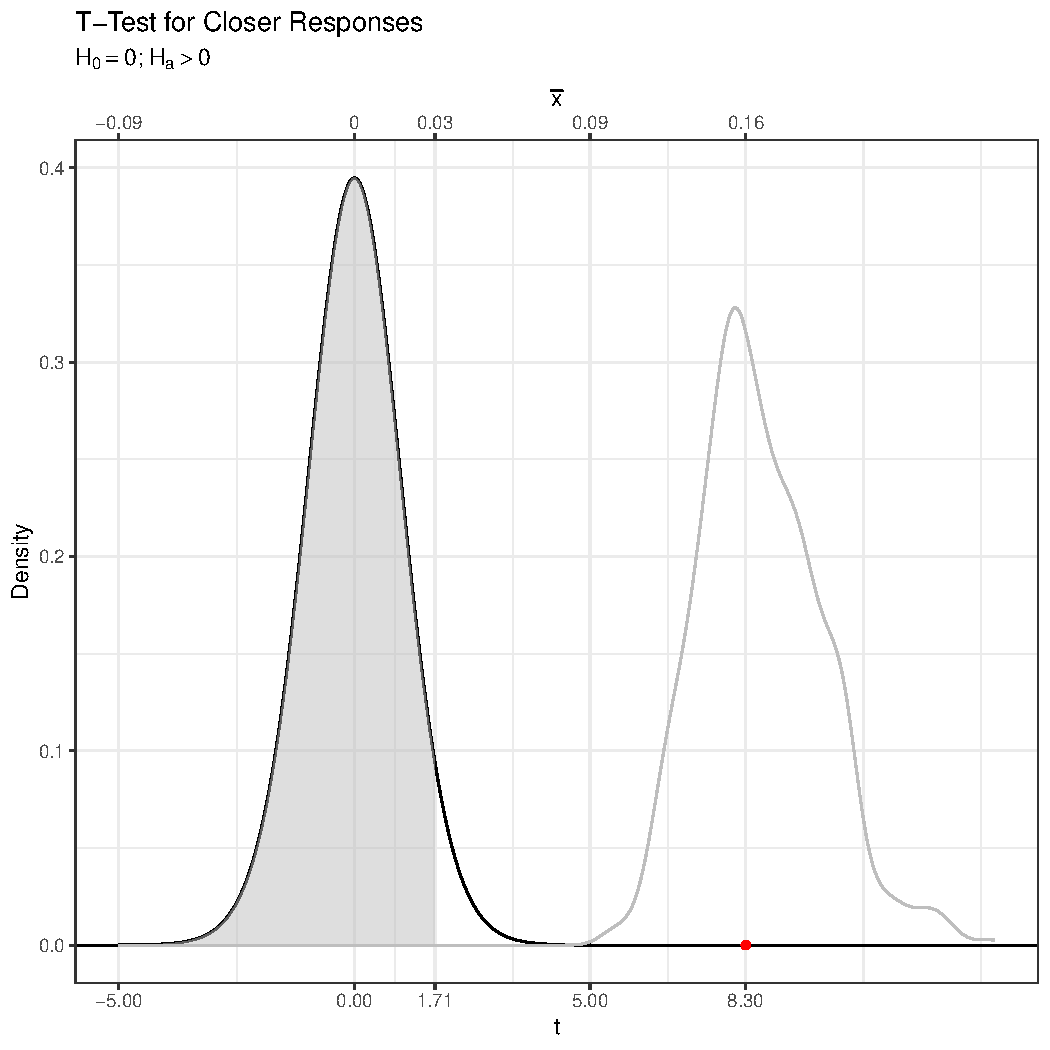
\includegraphics[width=\maxwidth]{figure/plot2-1} 
\end{knitrout}

\begin{figure}[H]
\begin{center}

\caption{Hypothesis Test Plot for Close Responses}
\label{closehypothesis} %we can now reference plot1
\end{center}
\end{figure}
  
  \item Question 4, part(b).
  
  Figure \ref{furtherhypothesis} tests whether dopamine levels significantly decrease
  when zebra finches sing in a way that diverges from the adult song. The hypotheses
  are $H_0: \mu = 0$ and $H_a: \mu < 0$. Here, the observed t-statistic is $t=-7.78$,
  marked by the red point on the left tail of the null distribution. The left rejection
  region and p-value area are both shaded to emphasize the extremity of the observed
  statistic. The p-value is again extremely small as you can see by where the red dot is
  located in relation to the tail. This result is consistent with a strong decrease
  in dopamine activity when vocalizations are less accurate, reinforcing the idea of 
  negative reinforcement. The resampling distribution confirms the leftward shift
  and supports the conclusion that the observed t-statistic is unlikely under the null.
  
\begin{knitrout}\scriptsize
\definecolor{shadecolor}{rgb}{0.969, 0.969, 0.969}\color{fgcolor}
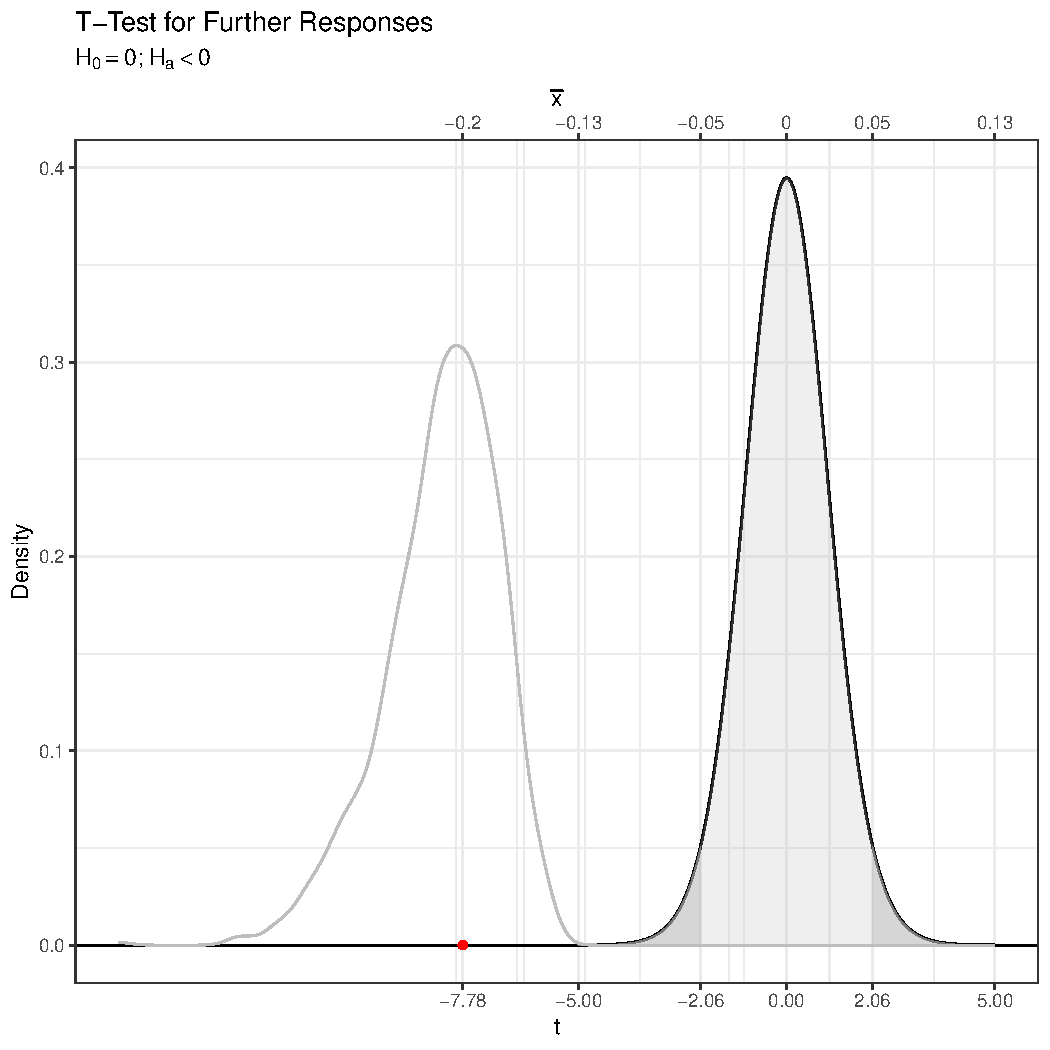
\includegraphics[width=\maxwidth]{figure/plot3-1} 
\end{knitrout}
  
  \begin{figure}[H]
\begin{center}

\caption{Hypothesis Test Plot for Far Responses}
\label{furtherhypothesis} %we can now reference plot1
\end{center}
\end{figure}
  
  
  \item Question 4, part(c).
  
  Figure \ref{differencehypothesis} compares dopamine responses directly between
  close and far vocalizations, testing the hypothesis $H_0: \mu = 0$ versus
  $H_a: \mu \neq 0$. The null distribution assumes no difference in percent
  fluorescence change between the two conditions. The observed t-statistic falls
  significantly to the right, $t=8.51$, indicating that dopamine responses are 
  markedly stronger when the zebra finches produce closer approximations to the
  adult song. The p-value is again essentially zero, supporting a statistically
  discernable difference between close and far responses. This plot emphasizes
  that dopamine not only increases during accurate vocalizations but does so
  significantly more than during inaccurate ones-- further reinforcing its role
  as a reinforcement signal during song learning.
  
\begin{knitrout}\scriptsize
\definecolor{shadecolor}{rgb}{0.969, 0.969, 0.969}\color{fgcolor}
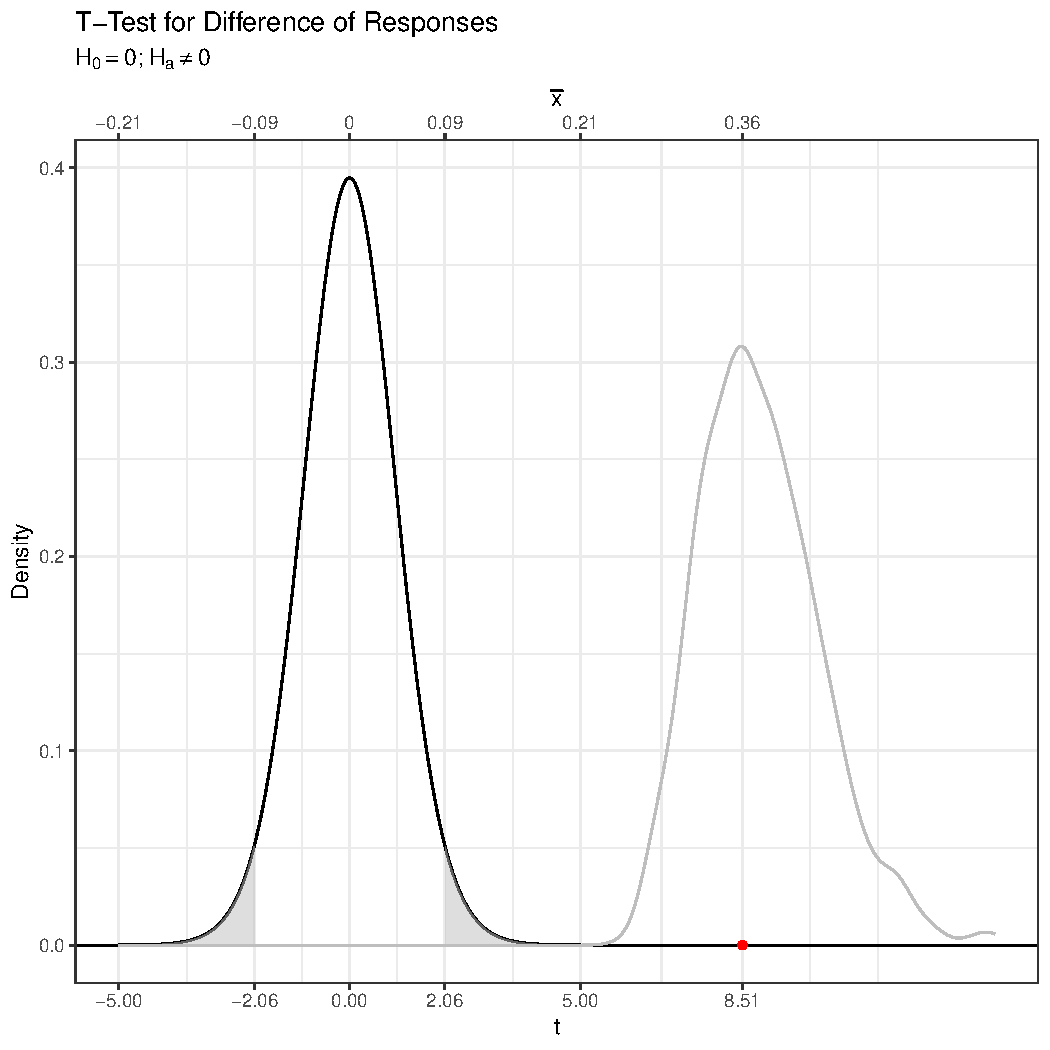
\includegraphics[width=\maxwidth]{figure/plot4-1} 
\end{knitrout}

  \begin{figure}[H]
\begin{center}

\caption{Hypothesis Test Plot for Difference Between Populations}
\label{differencehypothesis} %we can now reference plot1
\end{center}
\end{figure}
  
  
\end{enumerate}
\end{enumerate}


\bibliography{bibliography}
\end{document}
